
\chapter{绪论}
\label{chap:introduction}
\section{研究背景与意义}
	自互联网诞生以来,用户寻找信息的方法经历了几个阶段。早期的用户主要靠直接记住感兴趣网站的网址来寻找内容,直接促使Yahoo!提出了分类目录系统,将网站分门别类方便用户查询。但随着信息越来越多,分类目录也只能记录少量的网站,于是产生了搜索引擎。以Google为代表的搜索引擎可以让用户通过关键词找到自己需要的信息,但是,搜索引擎需要用户主动的提供显式关键词来寻找信息,因此它不能解决用户的更多的潜在需求,当用户无法精准描述自己的需求时,搜索引擎就无能为力了,于是又催生出推荐系统\citep{recmd-system}。以亚马逊电商官网为代表的推荐系统是一种帮助用户快速发现有用信息的工具,和搜索引擎不同的是推荐系统不需要提供明确的需求,而是通过分析用户的历史行为来给用户画像建模从而主动给用户推荐出能够满足他们兴趣和需求的信息。因此,从某种意义上说推荐系统和搜索引擎是两个互补的工具。搜索引擎满足用户显式的需求,而推荐系统能够在用户没有明确目的的时候帮助他们发现潜在的需要。随着物联网和用户终端设备的发展,人们逐渐从信息的匮乏时代走进了信息的过载(Information overload)时代。无论是作为信息消费者的普通用户,还是作为信息生产者的提供商面临着数据爆炸时代的挑战。作为用户,如何从充斥着大量噪声的大数据中找到自己感兴趣的信息是一件非常耗时费力的事情,笔者曾有过这样的一种购物体验:在淘宝商城购买一台笔记本电脑,花费了一上午的时间才浏览、比较完所有的 thinkpad 品牌商家店面,如\autoref{fig:hl_taobao}。而近年来淘宝的交易额增长规模巨大,2005年淘宝交易额为80亿,2010年为4000亿,而到2015年淘宝双十一单日交易额就为912亿元,可见未来几年内笔者的这种关键字搜索+逐条浏览的购物方式已经不再具有可行性。而作为提供商,如何让自己生产的信息不埋没在大数据洪流中而受到潜在用户的充分关注,这也是其所要解决的一个课题,很多企业已经或者正在开发适合本公司的推荐系统(Recommender System)来解决这一矛盾。

	推荐系统广泛应用于电子商务领域,通过分析用户的数据,帮助用户找到喜欢和感兴趣的商品,然后推荐给他们。推荐系统的最大优点在于它能收集用户的兴趣信息并根据用户的不同偏好,主动的为用户做出个性化推荐,而且此推荐信息是动态更新的,也就是说随着时间的推移,用户的兴趣在逐渐改变,推荐系统的推荐结果也会随之改变。因此,推荐系统大大的提高了网站的用户体验,方便了用户对资源信息的查询。推荐系统的主要任务就是联系用户和信息,一方面协助用户发现自己潜在感兴趣的信息从而提升用户的满意度,另一方面让信息针对性的展现在只对它有兴趣的用户面前从而提升商品的转化率,于是实现了消费者和生产者的双赢。
	\begin{figure}
		\centering
		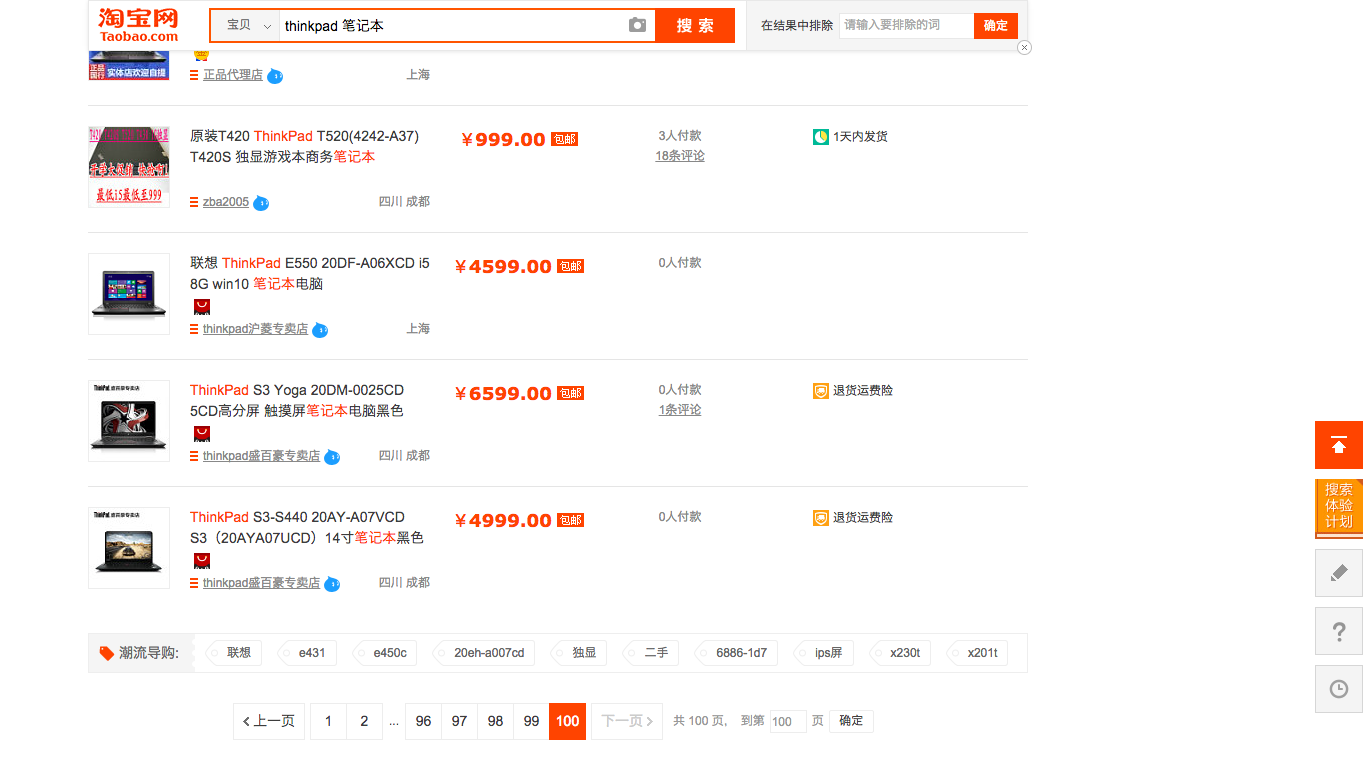
\includegraphics[width=0.9\textwidth]{hl_taobao}
		\figcaption{淘宝购物页面}
		\label{fig:hl_taobao}
	\end{figure}


	\subsection{推荐系统的产生与发展}
	随着科学技术与信息传播的迅猛发展,人类社会进入了一个全新的大数据时代,互联网和物联网无处不在的影响着人类生活的方方面面,并颠覆性改变了人们的生活方式,互联网用户既代表了网络信息的消费者,也代表了网络内容的生产者。尤其是随着Web 2.0时代的到来,社交化网络媒体的异军突起,互联网中的信息量呈指数级增长,而由于用户的辨别能力有限,使得其在庞大且复杂的互联网信息中找寻有用信息的成本巨大,这就是所谓的“信息过载问题。搜索引擎和推荐系统的出现为用户解决“信息过载提供了非常重要的技术手段。搜索引擎是被动的,用户在搜索互联网中的信息时需要在搜索引擎中输入关键词,搜索引擎根据输入在系统后台进行信息匹配,将与用户查询相关的信息展示给用户。但是当用户无法精确描述自己需求时,搜索引擎就无能为力了。推荐系统是主动的,用户不需要提供明确的需求,而是通过分析用户的历史行为来对用户进行分析,从而主动给用户推荐可能满足他们兴趣和需求的信息。因此搜索引擎和推荐系统是两个互补的技术手段。

	推荐系统概念是1995年在美国人工智能协会(AAAI)上由CMU大学的教授Robert Armstrong首先提出并推出了推荐系统的原型系统——Web Watcher。随后推荐系统的研究工作开始慢慢壮大。第一个正式商用的推荐系统是1996年Yahoo网站推出的个性化入口MyYahoo。21新世纪推荐系统的研究与应用随着电子商务的快速发展而风起云涌,各大电子商务网站都开发、部署了推荐系统,有报告称Amazon网站中35\%的营业额来自于自身的推荐系统。2006年美国的DVD租赁公司Netflix在网上公开设立了一个推荐算法竞赛并公开了真实网站中的一部分数据,包含用户对电影的评分。Netflix竞赛有效地推动了学术界和产业界对推荐算法的兴趣,很多有效的算法在此阶段被提了出来。近几年随着社会化网络的发展,推荐系统在工业界广泛应用并且取得了显著进步。比较著名的推荐系统应用有:淘宝网的电子商务推荐系统、Youtube的视频推荐系统、网易云音乐推荐系统以及Facebook好友推荐系统。

	自推荐系统诞生后学术界对其关注的兴趣度也越来越大。从1999年开始美国计算机学会每年召开电子商务研讨会以来,发表的与推荐系统相关的论文数以千计。ACM信息检索专业组在2001年开始把推荐系统作为该会议的一个独立研究主题。同年召开的人工智能联合大会也将推荐系统作为一个单独的主题。目前为止数据库、数据挖掘、人工智能、机器学习方面的重要国际会议(如KDD、AAAI、ICML等)都有大量与推荐系统相关的研究成果发表。同时第一个以推荐系统命名的国际会议ACM Recommender Systems Conference 于2007年首次举办。在近几年的数据挖掘及知识发现国际会议举办的竞赛中,连续两年的竞赛主题都是推荐系统。2011年的KDD CUP 竞赛中,两个竞赛题目分别为音乐评分预测和识别音乐是否被用户评分。2012年的KDD CUP 竞赛中,两个竞赛题目分别为腾讯微博中的好友推荐和计算广告中的点击率预测。

	\subsection{推荐系统与电子商务}
	近几年随着电子商务蓬勃发展,推荐系统在互联网中的优势地位也越来越明显。在国外比较著名的电子商务网站有Amazon和eBay,其中Amazon平台中采用的推荐算法是非常成功的。在国内比较典型的电子商务平台网站有淘宝网、网页云音乐、爱奇艺PPS等。在这些电子商务平台中,网站提供的商品数量不计其数,网站中的用户规模也非常巨大。据不完全统计天猫商城中的商品数量已经超过了5000万。在商品数量如此庞大的电商网站中,如果用户仅仅根据自己的购买意图输入关键字查询只会得到很多用户很难区分的相似结果,也不便用户做出选择。因此推荐系统作为能够根据用户兴趣为用户推荐商品的主要途径,从而为用户在购物的选择中提供建议的需求非常明显。目前比较成功的电子商务网站中,都不同程度地利用推荐系统在用户购物的同时为用户推荐一些商品,从而提高商品的销售额。另一方面,随着以智能手机为代表的物联网推动了移动互联网的发展。在用户在连入移动互联网的过程中,其所处的地理位置信息可以非常准确地被获取,并由此出现了大量的基于用户位置信息的网站。国外比较著名的有Uber和Coupons。国内著名的有滴滴出行和美团网。例如,在美团网这种基于位置服务的网站中,用户可以根据自己的当前位置搜索餐馆、酒店、影院、旅游景点等信息服务。同时,可以对当前位置下的各类信息进行点评,为自己在现实世界中的体验打分,分享自己的经验与感受。当用户使用这类基于位置的网站服务时,同样会遭遇“信息过载问题。推荐系统可以根据用户的位置信息为用户推荐当前位置下用户感兴趣的内容,为用户提供符合其真正需要的内容,提升用户对网站的满意度。

	随着社交网络的深入人心,用户在互联网中的行为不再局限于获取信息,更多的是与网络上的其他用户进行互动。国外著名的社交网络有Facebook、Twitter等,国内的社交网络有微信、米聊等。在社交网站中用户不再是单个的个体,而是与网络中的很多人具有了错综复杂的社交关系链。社交网络中最重要的资源就是用户与用户之间的这种联系。社交网络中用户间的关系是多维度的,建立社交关系的因素可能是在现实世界中是亲人、同学、同事、朋友关系,也可能只是网络中的虚拟朋友,比如都是有着共同爱好的会员成员。在社交网络中用户与用户之间的联系紧密度反映了用户之间的信任关系,用户不在是一个个体存在,其在社交网络中的行为或多或少地会受到其他用户关系的影响。因此推荐系统在这类社交网站中的研究与应用应该考虑用户社交的影响。

	现如今推荐系统在很多领域得到了广泛的应用,如出租车推荐、商品推荐、美餐推荐、电影推荐和音乐推荐,几乎囊括了人类的吃住行穿四大领域。不同领域的推荐系统具有不同的数据密度,对推荐系统的可扩展性以及推荐结果的相关性、流行性、新鲜性、多样性和新颖性具有不同的需求。

\section{推荐系统定义}
尽管实际需求不尽相同,一个完整的推荐系统通常都包括数据建模、用户建模、推荐引擎和用户接口4个部分,数据建模模块负责对拟推荐的物品数据进行准备,将其表示成有可以分析的数据格式,确定要推荐的候选物品集合,并对物品进行ETL、分类、聚类等预处理,数据建模模块是推荐系统的数据基础,也是最耗系统存储资源的部分。用户建模模块负责分析用户的行为数据并获得用户的潜在喜好。用户的行为信息包括购买、试用、下载、浏览、收藏、停留时间和评论等。推荐引擎模块利用后台的推荐算法,实时地从候选物品集合中筛选出用户感兴趣的物品,排序后以top N 的形式向用户提供推荐服务。推荐引擎是推荐系统的核心部分,也是最耗系统计算资源和时间的部分。用户接口模块承担展示推荐结果、收集用户反馈等功能。用户接口除了应具有布局合理、界面美观、使用方便等基本要求外,还要方便用户主动提供反馈。主要有两种类型的接口:Web端和移动端。接下来的章节会详细介绍用户建模和推荐引擎。
	\subsection{用户建模}
	用户模型反映了用户潜在的兴趣偏好。用户兴趣的反馈可分为显性反馈和隐性反馈。显性反馈包含用户定制和用户评分两种方式,其中,用户定制是指用户对系统所列问题的答复,如年龄、性别、职业等基本人口信息。评分又分为布尔评分和多维评分。例如在YahooNews中采用布尔评分:喜欢和不喜欢。多维评分可以更详细地描述对某个产品的喜欢程度,如滴滴出行中用户对司机提供的服务满意程度可评价为1~5分。

	很多时候用户不能够精准地提供个人偏好或者不愿意显性提供个人兴趣,更不愿意花费时间、精力维护个人的信息。所以隐性反馈往往能够正确地体现用户的偏好以及偏好的变化趋势。常用的隐性反馈信息有:浏览、点击、停留时长、点击时间、地点、收藏、评论内容、搜索内容和点击顺序等。在协同过滤推荐方法中常常利用用户的隐性反馈作为用户对产品的评分。例如小米手机主题应用中用户试用过的主题记为喜欢,评分为3;浏览过的主题记为感兴趣,评分为2,未浏览过的主题评分为1。一点资讯中用户点击了新闻标题评分为0.8分,阅读完全文则评分上升到1分;若用户跳过了系统推荐的新闻,则从系统预测评分中减去0.2分作为最终评分。

	用户的兴趣可分为长期兴趣和短期兴趣。长期兴趣反映用户的真实的兴趣,短期兴趣常与热点话题相结合且经常改动,从最近的用户行为中学习到的短期兴趣模型可快速反映用户兴趣的变化趋势。常用的模型有向量空间模型、隐式马尔科夫模型和基于分类器的模型等。由于用户的兴趣常受物品本身周期性、热点事件、突发事件的影响,随意性很大。所以需要用较短的时间频率来更新用户模型。

	\subsection{推荐引擎}
	从数学的角度来说,推荐模块的本质过程就是在给定的约束条件下,让用户的利益最大化的过程。对于一个推荐系统来说,将其模型化后,主要涉及到的变量集合有:系统中的用户集合U,系统中的产品项目集合I,用户集合和项目集合对应的偏好关系R,一般为评价集合,映射过程用效用函数f表示,即有:
	\begin{equation}
		f:U \times I \rightarrow R 
		\label{recmd_mapping}
	\end{equation}

	对于任意目标用户u,推荐系统的目的就是在项目空间I中搜索项目子集i,使得满足:
	 \begin{equation}
		N_{u}={max(f(u,N) | u\in U,N\in I)}
		\label{recmd_mapping}
	 \end{equation}

	推荐引擎的推荐方法可大致分为基于内容的推荐和基于协同过滤的推荐俩种。基于内容的推荐方法的原理是根据用户以往喜欢的物品,选择其他类似的物品作为推荐结果。例如现在有一部新电影与用户曾经看过的某部电影有相同演员或者标签类似,则用户有可能喜欢这部新电影。通常使用用户模型的标签向量空间来描述用户的兴趣偏好,同样对于每个物品的内容进行特征提取,作为物品模型的标签向量空间。然后计算用户模型的标签向量空间和候选物品模型的标签向量空间两者之间的相似度,相似度高的top N 候选物品就可作为推荐结果推送给目标用户。1992年提出的协同过滤技术是目前个性化推荐系统中应用最为成功和广泛的技术。国外的商业网站Amazon 和国内的网易云音乐网站,都采用了协同过滤技术。其本质是基于用户或商品关联分析的技术,即利用用户所在群体的共同喜好来向单个用户进行推荐。协同过滤利用了用户的历史行为数据将用户聚为一类,协同过滤推荐通过计算相似用户,假设其他相似用户喜好的物品,当前用户也会喜欢。基于用户的协同过滤推荐通常包括两个步骤:根据用户行为数据找到和目标用户兴趣相似的用户集,找到这个集合中用户喜欢的且目标用户没有购买过的物品推荐给目标用户。实际使用中协同过滤技术面临的制约,一是数据稀疏问题,二是冷启动问题。基于用户是协同过滤需要利用用户和用户或者物品与物品之间的关联性进行推荐。最流行的基于邻居关系的协同过滤方法:首先找出与指定用户评价历史数据相近的邻居,根据这些邻居的行为来预测用户行为或者找出与查询物品类似的物品。这样做的前提假设是两个用户在一组物品上有相似的评价,那么他们对其他的物品也倾向于有相似的评价。协同过滤算法的关键是找寻用户的最近邻居。当数据稀疏时,用户购买过的物品很难重叠导致协同推荐的效果就不是很有效,解决办法是二度邻居的行为也可以对当前用户的决策行为构成影响。另外一些解决稀疏问题的方法是添加缺省值,或者采用迭代补全的方法先补充部分数值,在此基础上再进一步补充其他数值。此外还可以利用迁移学习方法弥补数据稀疏。在真实应用中由于商品数量规模巨大,数据稀疏的问题更加突出。数据稀疏性使协同过滤方法的效果受到制约。如何甄别出与数据稀疏程度相适应的推荐算法是非常有价值的研究课题。常用的协同过滤方法有两类:基于内存的方法和基于模型的方法,前者主要是通过用户与物品之间的关系直接导出推荐结果,后者需要找到一个合适的参数化模型间接导出推荐结果。

	\begin{itemize}
		\item 基于内存的协同过滤鉴别出与查询用户相似的用户,然后将这些用户对物品评分的均值作为该用户评分结果的估计值。与此类似,基于物品的协同过滤鉴别出与查询物品类似的物品,然后将这些物品的评分均值作为该物品预测结果的估计值。常用的计算加权平均值的算法有皮尔逊系数、矢量余弦、MSD。
		\item 基于模型的方法通过适合训练集的参数化模型来预测结果。它包括聚类方法、贝叶斯分类器、回归方法。基于聚类方法的基本思想是将相似的用户聚合成类,有助于解决数据稀疏性和计算复杂性问题。贝叶斯的基本思想是给定用户A其他的评分和其他用户评分情况下,计算每个可能评分值的条件概率,然后选择一个最大概率值的评分作为预测值。基于回归方法的基本思想是先利用线性回归模型学习物品之间评分的关系,然后根据这些关系预测用户对物品的评分。
	\end{itemize}
	
	基于内容的推荐方法和基于协同过滤的推荐方法各有其优缺点。现有的系统大部分是一种混合系统,它结合不同算法和模型的优点并克服它们的缺点,从而得到了较好的推荐效果。最近一类成功的基于模型的方法是基于低秩矩阵分解的方法将评价矩阵分解为若干个低秩的子矩阵,这些子矩阵的乘积能对原始矩阵进行某种程度的复原,从而可以评估出缺失值。基于低秩矩阵分解的方法从评分矩阵中抽取一组潜在的因子,并通过这些因子向量描述用户和物品。在电影领域,这些自动识别的因子可能对应一部电影的常见标签。矩阵分解能够对两类变量进行交互关系的预测。如果将因子分解模型应用到一个新的任务,针对新问题往往需要在原有因子分解基础上推导演化,实现新的模型和学习算法。例如SVD++、 STE、 FPMC和TimeSVD++模型都是针对特定问题在原有因子分解模型基础上做的改进,因此普通的因子分解模型具有较差的泛化能力。在模型优化学习算法方面,虽然对基本矩阵分解模型的学习已经有很多算法,如梯度下降、交替最小二乘法和变分贝叶斯,但是对于更多的业务模型,最多且最常用的模型是结合了基于内容的推荐方法和基于协同过滤的推荐方法的组合模型。

\section{大数据时代下的推荐系统}
	虽然推荐系统己经被成功运用在很多大型系统、网站,但是在当前大数据的时代下,推荐系统的面临的场景越来越复杂,推荐系统不仅需要解决传统的数据稀疏、冷启动和动态兴趣问题,还面临由大数据引发的更多、更复杂的实际问题,例如数以亿计的用户数目和海量用户同时访问推荐系统所造成的性能压力,使传统的基于单节点架构的推荐系统不再适用。同时Web 服务器处理系统请求在大数据集下变得越来越多,Web服务器响应速度缓慢制约了当前推荐系统为大数据集提供推荐。基于实时模式的推荐在大数据集下也面临着严峻考验,用户难以忍受超过秒级的推荐结果返回时间。传统推荐系统的单一数据库存储技术在大数据集下变得不再适用,急需一种对外提供统一接口、对内采用多种混合模式存储的存储架构来满足大数据集下各种数据文件的存储。并且传统推荐系统在推荐算法上采取的是单机节点的计算方式也不能满足海量用户行为数据的计算需求。大数据本身具有的复杂性、不确定性也给推荐系统带来诸多新的挑战,传统推荐系统的时间效率、空间效率和推荐准确度都遇到严重的瓶颈。
	\subsection{推荐系统的关键技术}
	分布式文件系统。传统的推荐系统技术主要处理小文件存储和少量数据计算,大多是面向服务器的架构,中心服务器需要收集用户的浏览记录、购买记录、评分记录等大量的交互信息来为单个用户定制个性化推荐。当数据规模过大,数据无法全部载入服务器内存时,就算采用外存置换算法和多线程技术,依然会出现I/O上的性能瓶颈,致使任务执行效率过低,产生推荐结果的时间过长。对于面向海量用户和海量数据的推荐系统,基于集中式的中心服务器的推荐系统在时间和空间复杂性上无法满足大数据背景下推荐系统快速变化的需求。大数据推荐系统采用基于集群技术的分布式文件系统管理数据。建立一种高并发、可扩展、能处理海量数据的大数据推荐系统架构是非常关键的,它能为大数据集的处理提供强有力的支持。Hadoop 的分布式文件系统架构是其中的典型。与传统的文件系统不同,数据文件并非存储在本地单一节点上,而是通过网络存储在多台节点上。并且文件的位置索引管理一般都由一台或几台中心节点负责。客户端从集群中读写数据时,首先通过中心节点获取文件的位置,然后与集群中的节点通信,客户端通过网络从节点读取数据到本地或把数据从本地写入节点。在这个过程中由HDFS来管理数据冗余存储、大文件的切分、中间网络通信、数据出错恢复等,客户端根据HDFS 提供的接口进行调用即可,非常方便。
	
	分布式计算框架。集群上实现分布式计算的框架很多,Spark 作为推荐算法并行化的依托平台,既是一种分布式的计算框架,也是一种新型的分布式计算编程模型,是一种常见的开源计算框架。其基于内存的MapReduce算法的核心思想是分而治之,把对大规模数据集的操作,分发给一个主节点管理下的各个分节点共同完成,然后通过整合各个节点的中间结果,得到最终结果。计算框架负责处理并行编程中分布式存储、工作调度、负载均衡、容错均衡、容错处理以及网络通信等复杂问题,把处理过程高度抽象为两个函数: map和reduce。map负责把任务分解成多个任务,reduce负责把分解后多任务处理的结果汇总起来。
	
	推荐算法并行化。大型企业所需的推荐算法要处理的数据量非常庞大,从TB级别到PB级甚至更高,腾讯Peacock主题模型分析系统需要进行高达十亿文档、百万词汇、百万主题的主题模型训练,仅一个百万词汇乘以百万主题的矩阵,其数据存储量已达3TB。面对如此庞大的数据,若采用传统串行推荐算法,时间开销太大。当数据量较小时,时间复杂度高的串行算法能有效运作,但数据量极速增加后,这些串行推荐算法的计算性能过低,无法应用于实际的推荐系统中。因此,面向大数据集的推荐系统从设计上就应考虑到算法的分布式并行化技术,使得推荐算法能够在海量的、分布式、异构数据环境下得以高效实现。

	\subsection{推荐系统面临的问题}
	特征提取问题。推荐系统的推荐对象种类丰富,例如新闻、博客等文本类对象,视频、图片、音乐等多媒体对象以及可以用文本描述的一些实体对象等。如何对这些推荐对象进行特征提取一直是学术界和工业界的热门研究课题。对于文本类对象,可以借助信息检索领域己经成熟的文本特征提取技术来提取特征。对于多媒体对象,由于需要结合多媒体内容分析领域的相关技术来提取特征,而多媒体内容分析技术目前在学术界和工业界还有待完善,因此多媒体对象的特征提取是推荐系统目前面临的一大难题。此外推荐对象特征的区分度对推荐系统的性能有非常重要的影响。目前还缺乏特别有效的提高特征区分度的方法。

	数据稀疏问题。现有的大多数推荐算法都是基于用户—物品协同过滤矩阵数据,数据的稀疏性问题主要是指用户—物品评分矩阵的稀疏性,即用户与物品的交互行为太少。一个大型网站可能拥有上亿数量级的用户和物品,用户评分数据总量在面对增长更快的“用户—物品评价矩阵”时,仍然表现出稀疏性,推荐系统研究中的经典数据集MovieLens的稀疏度仅4.5\%, Netflix百万大赛中提供的音乐数据集的稀疏度是1.2\%。这些都是已经处理过的数据集,实际上真实数据集的稀疏度都远远低于1\%。例如, Bibsonomy的稀疏度是0.35\%,Delicious的稀疏度是0.046\%,淘宝网数据的稀疏度甚至仅在0.01\%左右。根据经验,数据集中用户行为数据越多,推荐算法的精准度越高,性能也越好。若数据集非常稀疏,只包含极少量的用户行为数据,推荐算法的准确度会大打折扣,极容易导致推荐算法的过拟合,影响算法的性能。

	冷启动问题。冷启动问题是推荐系统所面临的最大问题之一。冷启动问题总的来说可以分为3类:系统冷启动问题、新用户问题和新物品问题。系统冷启动问题指的是由于数据过于稀疏,“用户—物品评分矩阵”的密度太低,导致推荐系统得到的推荐结果准确性极低。新物品问题是由于新的物品缺少用户对该物品的评分,这类物品很难通过推荐系统被推荐给用户,用户难以对这些物品评分,从而形成恶性循环,导致一些新物品始终无法有效推荐。新物品问题对不同的推荐系统影响程度不同:对于用户可以通过多种方式查找物品的网站,新物品问题并没有太大影响,如电影推荐系统等,因为用户可以有多种途径找到电影观看并评分;而对于一些推荐是主要获取物品途径的网站,新物品问题会对推荐系统造成严重影响。通常解决这个问题的途径是激励或者雇佣少量用户对每一个新物品进行评分。新用户问题是目前对现实推荐系统挑战最大的冷启动问题:当一个新的用户使用推荐系统时,他没有对任何项目进行评分,因此系统无法对其进行个性化推荐;即使当新用户开始对少量项目进行评分时,由于评分太少,系统依然无法给出精确的推荐,这甚至会导致用户因为推荐体验不佳而停止使用推荐系统。当前解决新用户问题主要是通过结合基于内容和基于用户特征的方法,掌握用户的统计特征和兴趣特征,在用户只有少量评分甚至没有评分时做出比较准确的推荐。

	\subsection{推荐系统开源项目介绍}
	工欲善其事,必先利器,关于大数据,有很多令人兴奋的事情,但如何分析、利用它也带来了很多困惑。好在开源观念盛行的今天,有一些在大数据领域领先的免费开源技术可供利用。
	\begin{itemize}
		\item Apache Hadoop:Hadoop是一个由Apache基金会所开发的分布式系统基础架构,是一种用于分布式存储和处理商用硬件上大型数据集的开源框架,可让各企业迅速从海量结构化和非结构化数据中获得洞察力。Hadoop的框架最核心的设计就是HDFS和MapReduce。HDFS为海量的数据提供了存储,则MapReduce为海量的数据提供了计算。HDFS有高容错性的特点,并且设计用来部署在低廉的硬件上;而且它提供高吞吐量来访问应用程序的数据,适合那些有着超大数据的应用程序。MapReduce 本身就是用于并行处理大数据集的软件框架,其根源是函数性编程中的 map 和 reduce 函数。它由两个可能包含有许多实例的操作组成。Map 函数接受一组数据并将其转换为一个键/值对列表,输入域中的每个元素对应一个键/值对。
		\item Hive:Hive是建立在 Hadoop 上的数据仓库基础构架。它提供了一系列的工具,可以用来进行数据提取转化加载,这是一种可以存储、查询和分析存储在Hadoop中的大规模数据的机制。Hive定义了简单的类SQL查询语言,称为HQL,它允许熟悉SQL的用户查询数据。同时,这个语言也允许熟悉 MapReduce 开发者的开发自定义的 mapper 和 reducer 来处理内建的 mapper 和 reducer 无法完成的复杂的分析工作,十分适合数据仓库的统计分析。
		\item Spark:Spark是加州大学伯克利分校所开源的类Hadoop的通用并行框架,Spark拥有 Hadoop 所具有的优点;但不同于 Hadoop 的是Job中间输出结果可以保存在内存中,从而不再需要读写HDFS,因此Spark能更好地适用于数据挖掘与机器学习等需要迭代的MapReduce的算法。
		\item Kafka: Kafka 是一种高吞吐量的分布式发布订阅消息系统,它可以处理消费者规模的网站中的所有用户行为流数据。这种用户行为流数据是在现代网络上的许多社会功能的一个关键因素。这些数据通常是由于吞吐量的要求而通过处理日志和日志聚合来解决。对于像Hadoop的一样的日志数据和离线分析系统,但又要求实时处理的限制,Kafka一个可行的解决方案。其目的是通过Hadoop的并行加载机制来统一线上和离线的消息处理,也是为了通过集群机来提供实时的消费。
	\end{itemize}

	\section{论文结构}
		本文的其余正文内容由以下章节组成:
		\begin{itemize}
			\item 第二章首先介绍了推荐系统基本概念和算法模型,包括数据挖掘算法\citep{date-mining}和信息提取技术\citep{info-retrieval}的应用,然后详细介绍了用户画像和用户兴趣探索。
			\item 第三章主要讨论了如何设计一个实际的动态长尾推荐系统,以及动态推荐系统的各个主要模块设计和需要遵守的设计原则。然后根据手机主题业务特点介绍了用户兴趣动态性,最后讨论了推荐系统的评测指标。
			\item 第四章主要讨论了用户画像建模,包括用户画像的数据来源,用户标签权重计算,以及用户画像建模方式。接下来从不同维度分解用户画像标签属性,最后列举了用户画像在实际生产中的应用场景,包括解决用户冷启动、用户兴趣多样性的问题,并给出了相关的实验结果及分析。
			\item 第五章主要讨论了如何利用用户兴趣探索跟踪用户动态并挖掘用户小众兴趣,从而提升推荐系统的长尾效应,文中给出了相关的实验结果及分析。
			\item 第六章是论文的结束语和展望,在对目前工作简要总结的基础上,提出了推荐系统下一步研究的任务和方向。
		\end{itemize}